\chapter{Plano de trabalho}\label{chap:chap3}

Neste capítulo apresenta-se o planeamento de tarefas, seus objetivos,
faseamento e metodologia de abordagem. No final será feita uma breve
apresentação das tecnologias e ferramentas escolhidas que permitirão
realizar as tarefas e cumprir os objetivos propostos.


\section{Tarefas, objetivos e metodologia de abordagem}

Para poder iniciar os trabalhos com uma rede \ecat\, será necessário,
naturalmente, ter uma rede provisória funcional onde se possa iniciar o
desenvolvimento do software de controlo. Para isto, está planeada a
montagem de uma pequena rede \ecat\ através de um PC como dispositivo
mestre e um \raspi\ como dispositivo escravo. De seguida, será desenvolvido
o código de baixo nível para os \arduino\ em conjunto com os módulos
\emph{EasyCAT} como dispositivos escravo. Esta rede de prototipagem
permitirá o desenvolvimento de uma parte substancial do código de controlo,
tanto do lado do mestre como do lado dos escravos. Do lado do \arduino\
o código deverá controlar a velocidade do motor e fazer a contagem dos
impulsos do encoder. Do lado do Raspberry, o programa focar-se á no 
controlo de movimento e sincronização dos mesmos, bem como eventual controlo
do estado do laser.

\subsection{Calendarização}
De forma a tornar mais percetível a calendarização de tarefas, criou-se
um gráfico do tipo \emph{Gantt}, mostrado na figura \ref{fig:gantt}. Este
aparece compacto, apenas com distribuição pelo diversos meses, pois a
distribuição por semana, embora esteja definida, gerava uma imagem muito
larga.

\begin{figure}[htp]
 \centering
 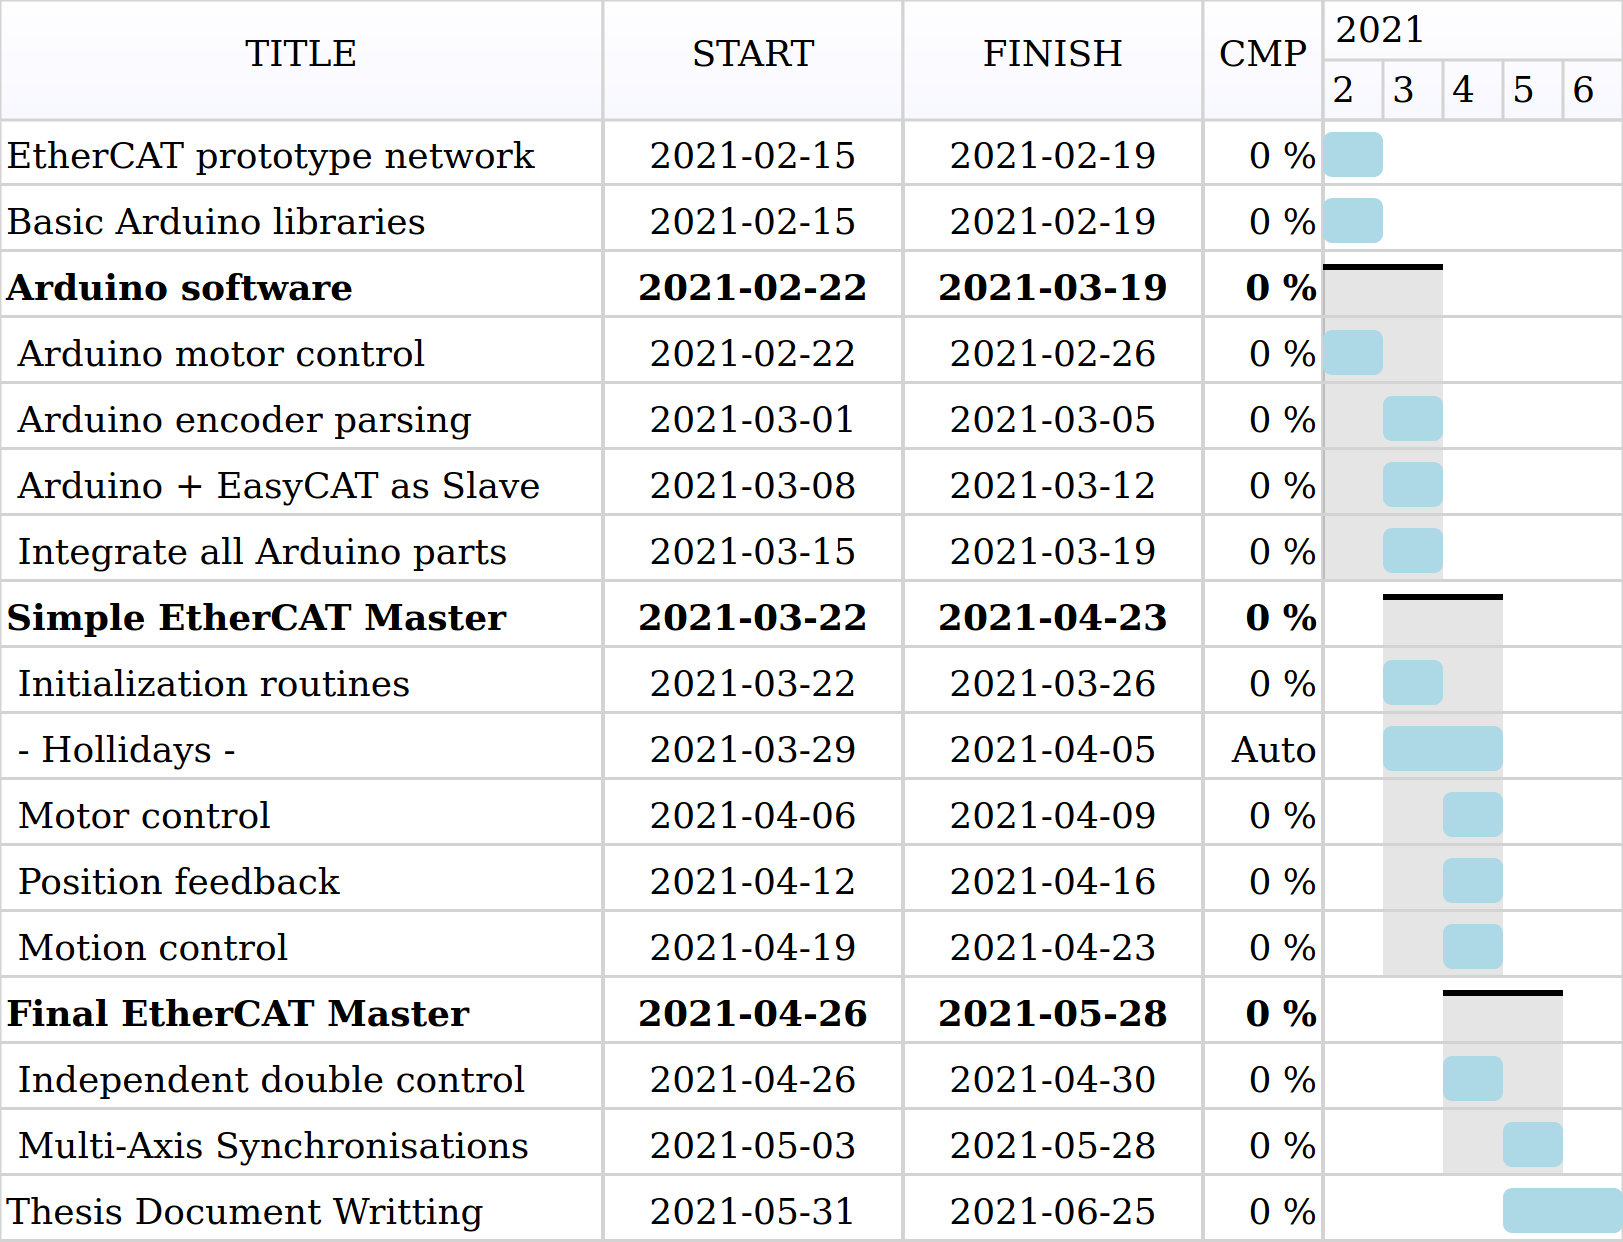
\includegraphics[width=0.86\textwidth]{Gantt.png}
 \caption{Diagrama de Gantt das tarefas propostas}
 \label{fig:gantt}
\end{figure}


\subsection{Tecnologias e ferramentas a usar}
Como descrito na secção \ref{sec:solution}, ir-se-á utilizar diversos
equipamentos para satisfazer requisitos diferentes, como por exemplo o
\raspi \cite[]{foundation:RaspberryPi} e dos \arduino. O primeiro será programado utilizando a plataforma 
\codesys\ \cite[]{CODESYS:codesys} que permite a utilização das linguagens
padrão da indústria de automação, IEC 61161-3. Os \arduino\ serão programados
em liguagem C, utilizando as librarias e compilador dedicados para os
micro-controladores AVR, que o \arduino\ utiliza. Para que este possa
funcionar como um escravo de \ecat, utilizar-se-á um adaptador \easycat\
da \cite{ABT:EasyCAT} e as respetivas librarias para desenvolver um
programa de controlo capaz de comandar a velocidade de rotação do motor
e de fazer a contagem de impulsos provenientes do codificador de posição.
O valor desta contagem deverá ser enviado para o \raspi\ de forma a que
este possa fazer o controlo de posição dos motores.

